% Created by tikzDevice version 0.12.6 on 2024-10-09 11:42:46
% !TEX encoding = UTF-8 Unicode
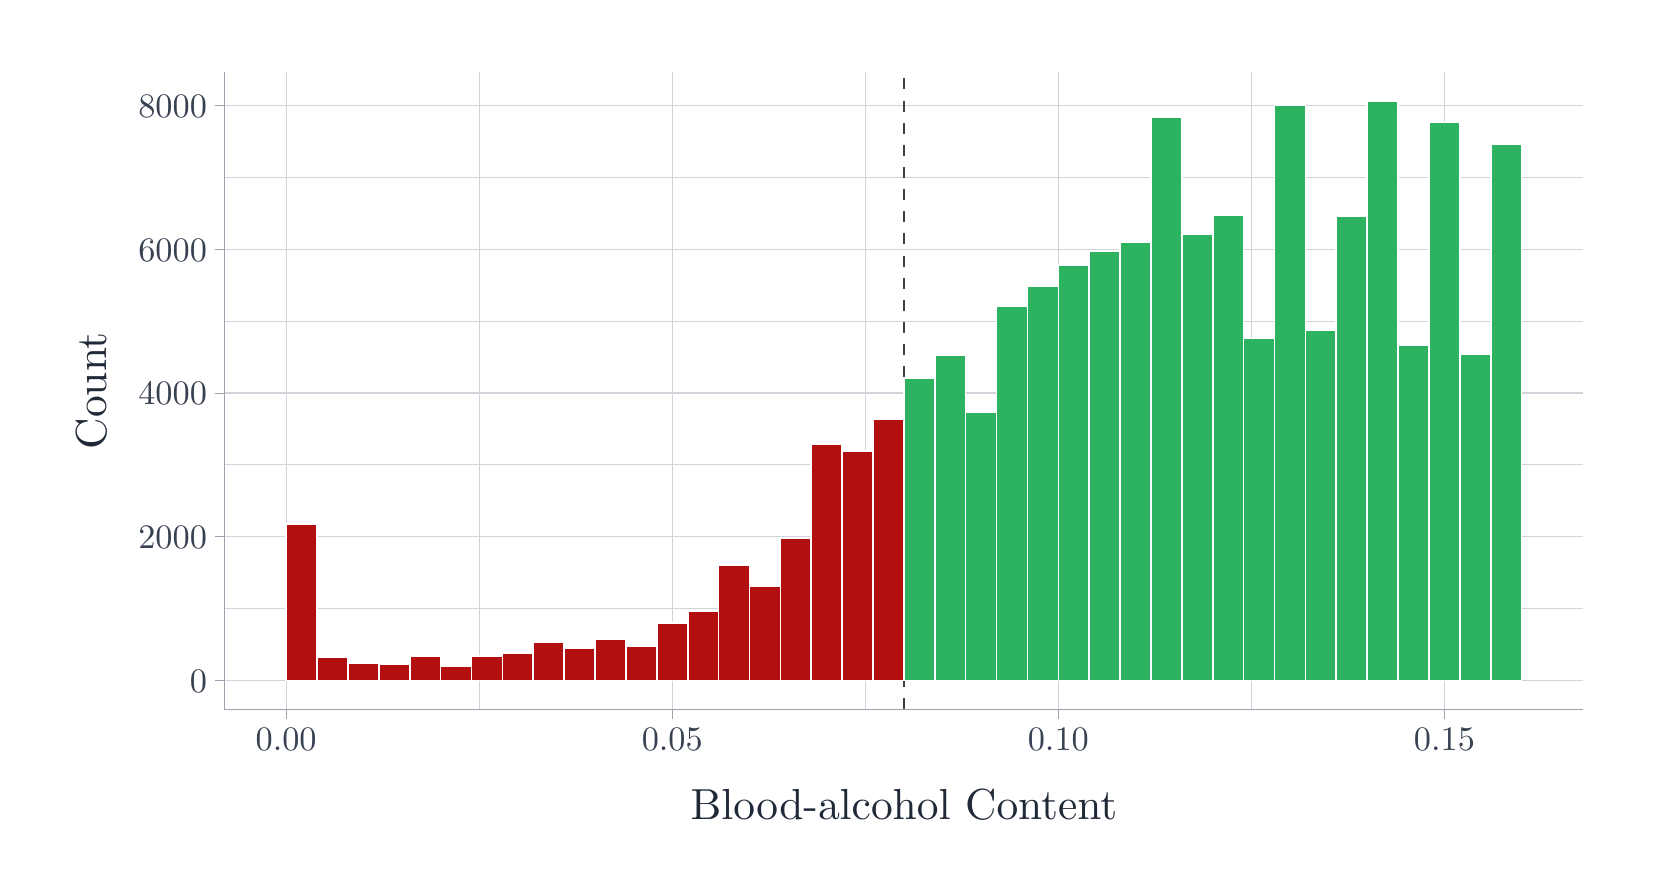
\begin{tikzpicture}[x=1pt,y=1pt]
\definecolor{fillColor}{RGB}{255,255,255}
\path[use as bounding box,fill=fillColor] (0,0) rectangle (578.16,303.53);
\begin{scope}
\path[clip] (  0.00,  0.00) rectangle (578.16,303.53);
\definecolor{drawColor}{RGB}{255,255,255}

\path[draw=drawColor,line width= 0.7pt,line join=round,line cap=round,fill=fillColor] (  0.00,  0.00) rectangle (578.16,303.53);
\end{scope}
\begin{scope}
\path[clip] ( 71.08, 57.20) rectangle (562.16,287.53);
\definecolor{drawColor}{RGB}{255,255,255}
\definecolor{fillColor}{RGB}{255,255,255}

\path[draw=drawColor,line width= 0.7pt,line join=round,line cap=round,fill=fillColor] ( 71.08, 57.20) rectangle (562.16,287.53);
\definecolor{drawColor}{RGB}{209,213,219}

\path[draw=drawColor,line width= 0.4pt,line join=round] ( 71.08, 93.63) --
	(562.16, 93.63);

\path[draw=drawColor,line width= 0.4pt,line join=round] ( 71.08,145.57) --
	(562.16,145.57);

\path[draw=drawColor,line width= 0.4pt,line join=round] ( 71.08,197.50) --
	(562.16,197.50);

\path[draw=drawColor,line width= 0.4pt,line join=round] ( 71.08,249.44) --
	(562.16,249.44);

\path[draw=drawColor,line width= 0.4pt,line join=round] (163.16, 57.20) --
	(163.16,287.53);

\path[draw=drawColor,line width= 0.4pt,line join=round] (302.67, 57.20) --
	(302.67,287.53);

\path[draw=drawColor,line width= 0.4pt,line join=round] (442.18, 57.20) --
	(442.18,287.53);

\path[draw=drawColor,line width= 0.4pt,line join=round] ( 71.08, 67.67) --
	(562.16, 67.67);

\path[draw=drawColor,line width= 0.4pt,line join=round] ( 71.08,119.60) --
	(562.16,119.60);

\path[draw=drawColor,line width= 0.4pt,line join=round] ( 71.08,171.53) --
	(562.16,171.53);

\path[draw=drawColor,line width= 0.4pt,line join=round] ( 71.08,223.47) --
	(562.16,223.47);

\path[draw=drawColor,line width= 0.4pt,line join=round] ( 71.08,275.40) --
	(562.16,275.40);

\path[draw=drawColor,line width= 0.4pt,line join=round] ( 93.40, 57.20) --
	( 93.40,287.53);

\path[draw=drawColor,line width= 0.4pt,line join=round] (232.92, 57.20) --
	(232.92,287.53);

\path[draw=drawColor,line width= 0.4pt,line join=round] (372.43, 57.20) --
	(372.43,287.53);

\path[draw=drawColor,line width= 0.4pt,line join=round] (511.94, 57.20) --
	(511.94,287.53);
\definecolor{drawColor}{RGB}{63,63,70}

\path[draw=drawColor,line width= 0.6pt,dash pattern=on 4pt off 4pt ,line join=round] (316.62, 57.20) -- (316.62,287.53);
\definecolor{drawColor}{RGB}{255,255,255}
\definecolor{fillColor}{RGB}{178,16,16}

\path[draw=drawColor,line width= 0.6pt,fill=fillColor] ( 93.40, 67.67) rectangle (104.57,124.20);

\path[draw=drawColor,line width= 0.6pt,fill=fillColor] (104.57, 67.67) rectangle (115.73, 75.92);

\path[draw=drawColor,line width= 0.6pt,fill=fillColor] (115.73, 67.67) rectangle (126.89, 73.92);

\path[draw=drawColor,line width= 0.6pt,fill=fillColor] (126.89, 67.67) rectangle (138.05, 73.59);

\path[draw=drawColor,line width= 0.6pt,fill=fillColor] (138.05, 67.67) rectangle (149.21, 76.29);

\path[draw=drawColor,line width= 0.6pt,fill=fillColor] (149.21, 67.67) rectangle (160.37, 72.88);

\path[draw=drawColor,line width= 0.6pt,fill=fillColor] (160.37, 67.67) rectangle (171.53, 76.47);

\path[draw=drawColor,line width= 0.6pt,fill=fillColor] (171.53, 67.67) rectangle (182.69, 77.48);

\path[draw=drawColor,line width= 0.6pt,fill=fillColor] (182.69, 67.67) rectangle (193.85, 81.32);

\path[draw=drawColor,line width= 0.6pt,fill=fillColor] (193.85, 67.67) rectangle (205.01, 79.22);

\path[draw=drawColor,line width= 0.6pt,fill=fillColor] (205.01, 67.67) rectangle (216.17, 82.65);

\path[draw=drawColor,line width= 0.6pt,fill=fillColor] (216.17, 67.67) rectangle (227.33, 79.97);

\path[draw=drawColor,line width= 0.6pt,fill=fillColor] (227.33, 67.67) rectangle (238.50, 88.36);

\path[draw=drawColor,line width= 0.6pt,fill=fillColor] (238.50, 67.67) rectangle (249.66, 92.57);

\path[draw=drawColor,line width= 0.6pt,fill=fillColor] (249.66, 67.67) rectangle (260.82,109.47);

\path[draw=drawColor,line width= 0.6pt,fill=fillColor] (260.82, 67.67) rectangle (271.98,101.63);

\path[draw=drawColor,line width= 0.6pt,fill=fillColor] (271.98, 67.67) rectangle (283.14,119.11);

\path[draw=drawColor,line width= 0.6pt,fill=fillColor] (283.14, 67.67) rectangle (294.30,152.92);

\path[draw=drawColor,line width= 0.6pt,fill=fillColor] (294.30, 67.67) rectangle (305.46,150.63);

\path[draw=drawColor,line width= 0.6pt,fill=fillColor] (305.46, 67.67) rectangle (316.62,162.21);

\path[draw=drawColor,line width= 0.6pt,fill=fillColor] (316.62,177.04) rectangle (327.78,177.04);

\path[draw=drawColor,line width= 0.6pt,fill=fillColor] (327.78,185.04) rectangle (338.94,185.04);

\path[draw=drawColor,line width= 0.6pt,fill=fillColor] (338.94,164.60) rectangle (350.10,164.60);

\path[draw=drawColor,line width= 0.6pt,fill=fillColor] (350.10,202.98) rectangle (361.26,202.98);

\path[draw=drawColor,line width= 0.6pt,fill=fillColor] (361.26,210.25) rectangle (372.43,210.25);

\path[draw=drawColor,line width= 0.6pt,fill=fillColor] (372.43,217.73) rectangle (383.59,217.73);

\path[draw=drawColor,line width= 0.6pt,fill=fillColor] (383.59,222.74) rectangle (394.75,222.74);

\path[draw=drawColor,line width= 0.6pt,fill=fillColor] (394.75,225.93) rectangle (405.91,225.93);

\path[draw=drawColor,line width= 0.6pt,fill=fillColor] (405.91,271.20) rectangle (417.07,271.20);

\path[draw=drawColor,line width= 0.6pt,fill=fillColor] (417.07,228.77) rectangle (428.23,228.77);

\path[draw=drawColor,line width= 0.6pt,fill=fillColor] (428.23,235.80) rectangle (439.39,235.80);

\path[draw=drawColor,line width= 0.6pt,fill=fillColor] (439.39,191.27) rectangle (450.55,191.27);

\path[draw=drawColor,line width= 0.6pt,fill=fillColor] (450.55,275.40) rectangle (461.71,275.40);

\path[draw=drawColor,line width= 0.6pt,fill=fillColor] (461.71,194.18) rectangle (472.87,194.18);

\path[draw=drawColor,line width= 0.6pt,fill=fillColor] (472.87,235.49) rectangle (484.03,235.49);

\path[draw=drawColor,line width= 0.6pt,fill=fillColor] (484.03,277.06) rectangle (495.19,277.06);

\path[draw=drawColor,line width= 0.6pt,fill=fillColor] (495.19,188.96) rectangle (506.36,188.96);

\path[draw=drawColor,line width= 0.6pt,fill=fillColor] (506.36,269.27) rectangle (517.52,269.27);

\path[draw=drawColor,line width= 0.6pt,fill=fillColor] (517.52,185.50) rectangle (528.68,185.50);

\path[draw=drawColor,line width= 0.6pt,fill=fillColor] (528.68,261.35) rectangle (539.84,261.35);
\definecolor{fillColor}{RGB}{45,178,95}

\path[draw=drawColor,line width= 0.6pt,fill=fillColor] ( 93.40, 67.67) rectangle (104.57, 67.67);

\path[draw=drawColor,line width= 0.6pt,fill=fillColor] (104.57, 67.67) rectangle (115.73, 67.67);

\path[draw=drawColor,line width= 0.6pt,fill=fillColor] (115.73, 67.67) rectangle (126.89, 67.67);

\path[draw=drawColor,line width= 0.6pt,fill=fillColor] (126.89, 67.67) rectangle (138.05, 67.67);

\path[draw=drawColor,line width= 0.6pt,fill=fillColor] (138.05, 67.67) rectangle (149.21, 67.67);

\path[draw=drawColor,line width= 0.6pt,fill=fillColor] (149.21, 67.67) rectangle (160.37, 67.67);

\path[draw=drawColor,line width= 0.6pt,fill=fillColor] (160.37, 67.67) rectangle (171.53, 67.67);

\path[draw=drawColor,line width= 0.6pt,fill=fillColor] (171.53, 67.67) rectangle (182.69, 67.67);

\path[draw=drawColor,line width= 0.6pt,fill=fillColor] (182.69, 67.67) rectangle (193.85, 67.67);

\path[draw=drawColor,line width= 0.6pt,fill=fillColor] (193.85, 67.67) rectangle (205.01, 67.67);

\path[draw=drawColor,line width= 0.6pt,fill=fillColor] (205.01, 67.67) rectangle (216.17, 67.67);

\path[draw=drawColor,line width= 0.6pt,fill=fillColor] (216.17, 67.67) rectangle (227.33, 67.67);

\path[draw=drawColor,line width= 0.6pt,fill=fillColor] (227.33, 67.67) rectangle (238.50, 67.67);

\path[draw=drawColor,line width= 0.6pt,fill=fillColor] (238.50, 67.67) rectangle (249.66, 67.67);

\path[draw=drawColor,line width= 0.6pt,fill=fillColor] (249.66, 67.67) rectangle (260.82, 67.67);

\path[draw=drawColor,line width= 0.6pt,fill=fillColor] (260.82, 67.67) rectangle (271.98, 67.67);

\path[draw=drawColor,line width= 0.6pt,fill=fillColor] (271.98, 67.67) rectangle (283.14, 67.67);

\path[draw=drawColor,line width= 0.6pt,fill=fillColor] (283.14, 67.67) rectangle (294.30, 67.67);

\path[draw=drawColor,line width= 0.6pt,fill=fillColor] (294.30, 67.67) rectangle (305.46, 67.67);

\path[draw=drawColor,line width= 0.6pt,fill=fillColor] (305.46, 67.67) rectangle (316.62, 67.67);

\path[draw=drawColor,line width= 0.6pt,fill=fillColor] (316.62, 67.67) rectangle (327.78,177.04);

\path[draw=drawColor,line width= 0.6pt,fill=fillColor] (327.78, 67.67) rectangle (338.94,185.04);

\path[draw=drawColor,line width= 0.6pt,fill=fillColor] (338.94, 67.67) rectangle (350.10,164.60);

\path[draw=drawColor,line width= 0.6pt,fill=fillColor] (350.10, 67.67) rectangle (361.26,202.98);

\path[draw=drawColor,line width= 0.6pt,fill=fillColor] (361.26, 67.67) rectangle (372.43,210.25);

\path[draw=drawColor,line width= 0.6pt,fill=fillColor] (372.43, 67.67) rectangle (383.59,217.73);

\path[draw=drawColor,line width= 0.6pt,fill=fillColor] (383.59, 67.67) rectangle (394.75,222.74);

\path[draw=drawColor,line width= 0.6pt,fill=fillColor] (394.75, 67.67) rectangle (405.91,225.93);

\path[draw=drawColor,line width= 0.6pt,fill=fillColor] (405.91, 67.67) rectangle (417.07,271.20);

\path[draw=drawColor,line width= 0.6pt,fill=fillColor] (417.07, 67.67) rectangle (428.23,228.77);

\path[draw=drawColor,line width= 0.6pt,fill=fillColor] (428.23, 67.67) rectangle (439.39,235.80);

\path[draw=drawColor,line width= 0.6pt,fill=fillColor] (439.39, 67.67) rectangle (450.55,191.27);

\path[draw=drawColor,line width= 0.6pt,fill=fillColor] (450.55, 67.67) rectangle (461.71,275.40);

\path[draw=drawColor,line width= 0.6pt,fill=fillColor] (461.71, 67.67) rectangle (472.87,194.18);

\path[draw=drawColor,line width= 0.6pt,fill=fillColor] (472.87, 67.67) rectangle (484.03,235.49);

\path[draw=drawColor,line width= 0.6pt,fill=fillColor] (484.03, 67.67) rectangle (495.19,277.06);

\path[draw=drawColor,line width= 0.6pt,fill=fillColor] (495.19, 67.67) rectangle (506.36,188.96);

\path[draw=drawColor,line width= 0.6pt,fill=fillColor] (506.36, 67.67) rectangle (517.52,269.27);

\path[draw=drawColor,line width= 0.6pt,fill=fillColor] (517.52, 67.67) rectangle (528.68,185.50);

\path[draw=drawColor,line width= 0.6pt,fill=fillColor] (528.68, 67.67) rectangle (539.84,261.35);
\end{scope}
\begin{scope}
\path[clip] (  0.00,  0.00) rectangle (578.16,303.53);
\definecolor{drawColor}{RGB}{156,163,175}

\path[draw=drawColor,line width= 0.3pt,line join=round] ( 71.08, 57.20) --
	( 71.08,287.53);
\end{scope}
\begin{scope}
\path[clip] (  0.00,  0.00) rectangle (578.16,303.53);
\definecolor{drawColor}{RGB}{55,65,81}

\node[text=drawColor,anchor=base east,inner sep=0pt, outer sep=0pt, scale=  1.24] at ( 64.78, 63.38) {0};

\node[text=drawColor,anchor=base east,inner sep=0pt, outer sep=0pt, scale=  1.24] at ( 64.78,115.32) {2000};

\node[text=drawColor,anchor=base east,inner sep=0pt, outer sep=0pt, scale=  1.24] at ( 64.78,167.25) {4000};

\node[text=drawColor,anchor=base east,inner sep=0pt, outer sep=0pt, scale=  1.24] at ( 64.78,219.18) {6000};

\node[text=drawColor,anchor=base east,inner sep=0pt, outer sep=0pt, scale=  1.24] at ( 64.78,271.12) {8000};
\end{scope}
\begin{scope}
\path[clip] (  0.00,  0.00) rectangle (578.16,303.53);
\definecolor{drawColor}{RGB}{156,163,175}

\path[draw=drawColor,line width= 0.3pt,line join=round] ( 67.58, 67.67) --
	( 71.08, 67.67);

\path[draw=drawColor,line width= 0.3pt,line join=round] ( 67.58,119.60) --
	( 71.08,119.60);

\path[draw=drawColor,line width= 0.3pt,line join=round] ( 67.58,171.53) --
	( 71.08,171.53);

\path[draw=drawColor,line width= 0.3pt,line join=round] ( 67.58,223.47) --
	( 71.08,223.47);

\path[draw=drawColor,line width= 0.3pt,line join=round] ( 67.58,275.40) --
	( 71.08,275.40);
\end{scope}
\begin{scope}
\path[clip] (  0.00,  0.00) rectangle (578.16,303.53);
\definecolor{drawColor}{RGB}{156,163,175}

\path[draw=drawColor,line width= 0.3pt,line join=round] ( 71.08, 57.20) --
	(562.16, 57.20);
\end{scope}
\begin{scope}
\path[clip] (  0.00,  0.00) rectangle (578.16,303.53);
\definecolor{drawColor}{RGB}{156,163,175}

\path[draw=drawColor,line width= 0.3pt,line join=round] ( 93.40, 53.70) --
	( 93.40, 57.20);

\path[draw=drawColor,line width= 0.3pt,line join=round] (232.92, 53.70) --
	(232.92, 57.20);

\path[draw=drawColor,line width= 0.3pt,line join=round] (372.43, 53.70) --
	(372.43, 57.20);

\path[draw=drawColor,line width= 0.3pt,line join=round] (511.94, 53.70) --
	(511.94, 57.20);
\end{scope}
\begin{scope}
\path[clip] (  0.00,  0.00) rectangle (578.16,303.53);
\definecolor{drawColor}{RGB}{55,65,81}

\node[text=drawColor,anchor=base,inner sep=0pt, outer sep=0pt, scale=  1.24] at ( 93.40, 42.33) {0.00};

\node[text=drawColor,anchor=base,inner sep=0pt, outer sep=0pt, scale=  1.24] at (232.92, 42.33) {0.05};

\node[text=drawColor,anchor=base,inner sep=0pt, outer sep=0pt, scale=  1.24] at (372.43, 42.33) {0.10};

\node[text=drawColor,anchor=base,inner sep=0pt, outer sep=0pt, scale=  1.24] at (511.94, 42.33) {0.15};
\end{scope}
\begin{scope}
\path[clip] (  0.00,  0.00) rectangle (578.16,303.53);
\definecolor{drawColor}{RGB}{31,41,55}

\node[text=drawColor,anchor=base,inner sep=0pt, outer sep=0pt, scale=  1.57] at (316.62, 17.53) {Blood-alcohol Content};
\end{scope}
\begin{scope}
\path[clip] (  0.00,  0.00) rectangle (578.16,303.53);
\definecolor{drawColor}{RGB}{31,41,55}

\node[text=drawColor,rotate= 90.00,anchor=base,inner sep=0pt, outer sep=0pt, scale=  1.57] at ( 28.38,172.36) {Count};
\end{scope}
\end{tikzpicture}
